\section{Casi d'uso} \label{section:casi_uso}

\subsection{Scopo}
Lo scopo di questa sezione è la descrizione in elenco di tutti i casi d'uso individuati dal gruppo, in
riferimento alle funzionalità dell'applicazione.

\subsection{Attori}
Come accordato con il proponente, la web app\glo{} deve essere usata sia dal venditore che dall'acquirente,
sono quindi presenti differenti attori nella gerarchia: 
\begin{itemize}
    \item La piattaforma e-commerce\glo{} da cui parte l'ordine,
    \item Metamask\glo{}
    \item L'utente generico che si divide in:
        \begin{itemize}
            \item Acquirente,
            \item Venditore;
        \end{itemize}
    \item L'acquirente che inizializza un ordine di qualsiasi tipo è il Proprietario Ordine;
    \item L'acquirente che inizializza un ordine scegliendo la tipologia di pagamento MoneyBox è il Proprietario MoneyBox;
    \item Infine ogni acquirente che dispone di un invito di partecipazione ad una MoneyBox è un Partecipante MoneyBox.
\end{itemize}}

\begin{figure}[H]
    \centering
    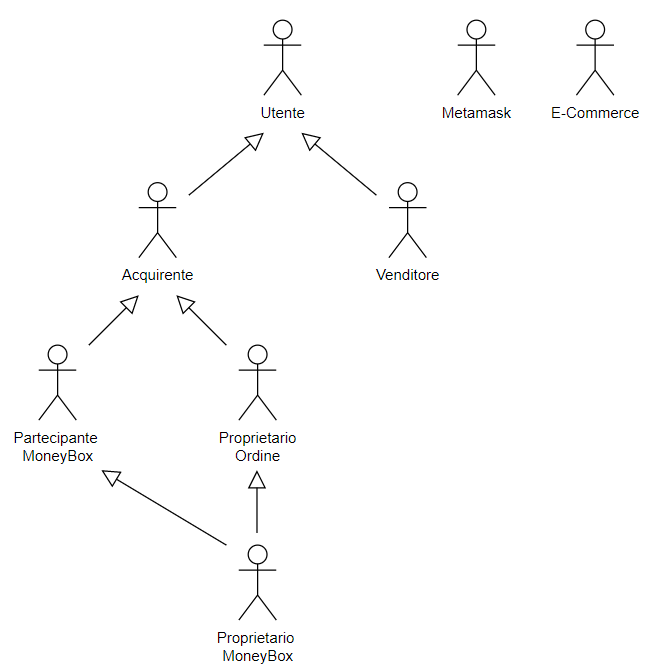
\includegraphics[scale=0.7]{immagini/Attori.png}
    \caption{Diagramma degli attori}
\end{figure}

\subsection{UC1 - Inizializzazione della Transazione}\label{subsection: UC1}

\begin{figure}[H]
    \centering
    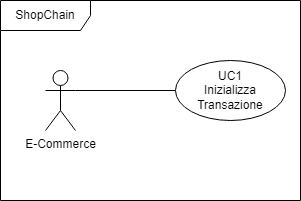
\includegraphics[scale=0.7]{immagini/UC1.png}
    \caption{UC1}
\end{figure}

\begin{itemize}
    \item Attore primario: e-commerce\glo{};
    \item Precondizioni: il sistema è raggiungibile e funzionante;
    \item Postcondizioni: la transazione viene caricata nel sistema, l'utente viene reindirizzato alla pagina di checkout;
    \item Scenario principale: L'e-commerce\glo{} delega il pagamento comunicando la somma richiesta e l'indirizzo del destinatario.
\end{itemize}

\subsection{UC2 - Checkout}\label{subsection: UC2}

\begin{figure}[H]
    \centering
    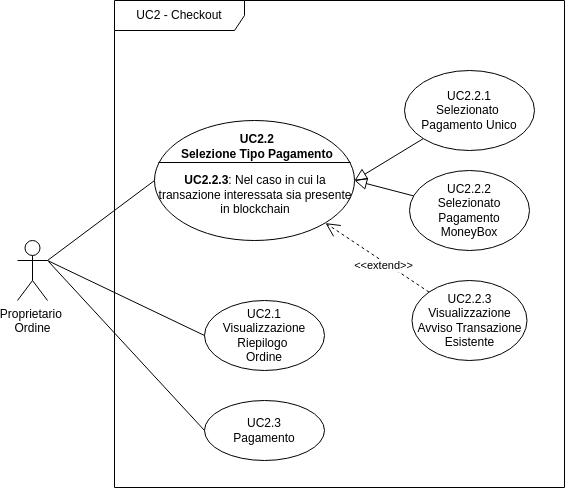
\includegraphics[scale=0.7]{immagini/UC2.png}
    \caption{UC2}
\end{figure}

\begin{itemize}
    \item Attore primario: Utente proprietario dell'ordine, acquirente;
    \item Precondizioni: l'e-commerce\glo{} ha iniziato la transazione [UC1];
    \item Postcondizioni: viene visualizzato l'esito dell'operazione;
    \item Scenario principale:
    \begin{enumerate}
        \item L'acquirente visualizza il riepilogo dell'ordine [UC2.1];
        \item Il proprietario dell'ordine seleziona la tipologia di pagamento tra quelle disponibili [UC2.2];
        \item L'acquirente effettua il pagamento [UC2.3];
        \item Se le condizioni sono soddisfatte il proprietario dell'ordine visualizza il codice di sblocco.
    \end{enumerate}
\end{itemize}

\subsubsection{UC2.1 - Visualizzazione Riepilogo Ordine}\label{sssec: UC2.1}

\begin{itemize}
    \item Attore primario: acquirente;
    \item Precondizioni: l'e-commerce\glo{} ha iniziato la transazione [UC1];
    \item Postcondizioni: l'acquirente ha visualizzato il riepilogo dell'ordine;
    \item Scenario principale:
          \begin{enumerate}
              \item L'acquirente visualizza il totale dell'ordine;
              \item L'acquirente visualizza l'indirizzo del venditore.
          \end{enumerate}
\end{itemize}

\subsubsection{UC2.2 - Selezione Tipo Pagamento}\label{sssec: UC2.2}

\begin{itemize}
    \item Attore primario: utente proprietario dell'ordine;
    \item Precondizioni: l'e-commerce\glo{} ha iniziato la transazione [UC1];
    \item Postcondizioni: il proprietario dell'ordine ha selezionato un metodo di pagamento;
    \item Scenario principale: il proprietario dell'ordine seleziona la tipologia di pagamento obbligando i successivi pagamenti per questa transazione alla tipologia scelta;
    \item Estensioni:
    \begin{enumerate}
    \item Nel caso in cui, per la transazione interessata, sia già stata scelta la tipologia di pagamento e quindi risultasse presente in blockchain\glo{}:
        \begin{itemize}
            \item La selezione della tipologia di pagamento viene omessa;
            \item Viene visualizzato Avviso Transazione Esistente [UC2.2.3].
        \end{itemize}
    \end{enumerate}
    \item Generalizzazioni:
    \begin{itemize}
        \item Selezionato Pagamento Unico [UC2.2.1];
        \item Selezionato Pagamento MoneyBox\glo{} [UC2.2.2].
    \end{itemize}
\end{itemize}

\paragraph{UC2.2.1 - Selezionato Pagamento Unico}\label{sssec: UC2.2.1}

\begin{itemize}
    \item Attore primario: utente proprietario dell'ordine;
    \item Precondizioni: l'e-commerce\glo{} ha iniziato la transazione [UC1];
    \item Postcondizioni: il proprietario dell'ordine ha selezionato pagamento unico come metodo di pagamento;
    \item Scenario principale: 
        \begin{itemize}
            \item Il proprietario dell'ordine seleziona pagamento unico come metodo di pagamento;
            \item Viene vincolato il successivo pagamento per questa transazione ad un pagamento unico della somma totale dovuta (UC2.3.1), il quale potrà essere effettuato dal proprietario dell'ordine.
        \end{itemize}}
\end{itemize}

\paragraph{UC2.2.2 - Selezionato Pagamento MoneyBox}

\begin{itemize}
    \item Attore primario: utente proprietario dell'ordine;
    \item Precondizioni: l'e-commerce\glo{} ha iniziato la transazione [UC1];
    \item Postcondizioni: il proprietario dell'ordine ha selezionato pagamento MoneyBox\glo{} come metodo di pagamento;
    \item Scenario principale: 
        \begin{itemize}
            \item Il proprietario dell'ordine seleziona pagamento MoneyBox\glo{} come metodo di pagamento;
            \item Viene creata la MoneyBox;
            \item Vengono vincolati i successivi pagamenti per questa transazione ad un pagamento parziale della somma totale rimanente (UC2.3.2), i quali potranno essere effettuati da un qualsiasi partecipante MoneyBox\glo{}.
        \end{itemize}} 
\end{itemize}

\paragraph{UC2.2.3 - Visualizzazione avviso transazione esistente}

\begin{itemize}
    \item Attore primario: utente proprietario dell'ordine;
    \item Precondizioni: l'e-commerce\glo{} ha iniziato la transazione [UC1], transazione già presente in blockchain;
    \item Postcondizioni: il proprietario dell'ordine ha visualizzato il messaggio di avviso transazione esistente;
    \item Scenario principale: il proprietario dell'ordine visualizza il messaggio di avviso, poiché la transazione è già presente in blockchain\glo{}.
\end{itemize}

\subsubsection{UC2.3 - Pagamento}

\begin{figure}[H]
    \centering
    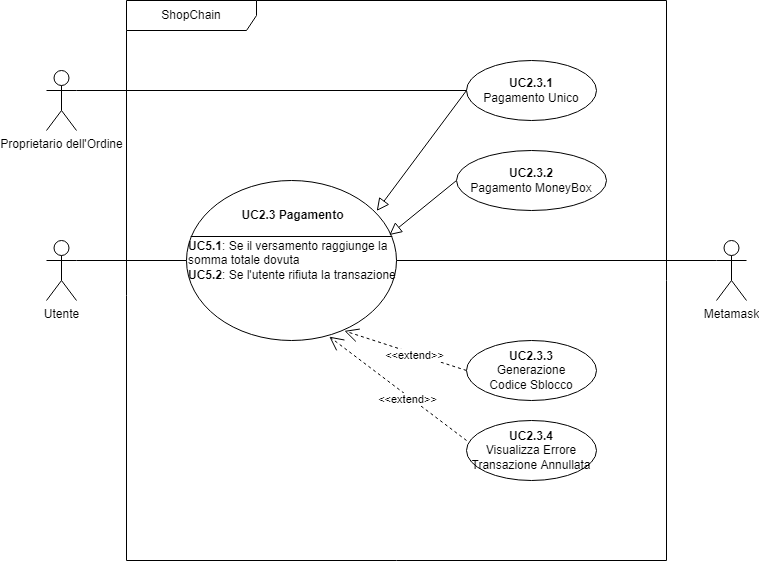
\includegraphics[scale=0.7]{immagini/UC2.3.png}
    \caption{UC2.3}
\end{figure}

\begin{itemize}
    \item Attore primario: acquirente;
    \item Attore secondario: Metamask\glo{};
    \item Precondizioni: è stata selezionata una tipologia di pagamento per la transazione interessata dal proprietario dell'ordine [UC2.2], 
            l'acquirente ha connesso il proprio wallet\glo{} tramite Metamask\glo{} [UC4];
    \item Postcondizioni: l'acquirente ha effettuato il pagamento;
    \item Scenario principale:
          \begin{enumerate}
              \item L'acquirente visualizza il pop-up di Metamask\glo{} con i dettagli della transazione;
              \item L'acquirente visualizza un overlay di caricamento sulla pagina di ShopChain;
              \item L'acquirente autorizza la transazione per l'importo impostato a seconda della tipologia precedentemente scelta dal proprietario dell'ordine (in UC2.2);
              \item L'acquirente visualizza un messaggio di conferma di avvenuto pagamento.
          \end{enumerate}
    \item Estensioni:
          \begin{enumerate}
              \item Nel caso l'acquirente rifiuti il pagamento:
              \begin{itemize}
                  \item La transazione viene annullata;
                  \item L'acquirente visualizza errore transazione annullata [UC2.3.3].
              \end{itemize}
          \end{enumerate}
    \item Generalizzazioni:
          \begin{enumerate}
              \item Pagamento Unico [UC2.3.1];
              \item Pagamento MoneyBox\glo{} [UC2.3.2].
          \end{enumerate}
\end{itemize}

\paragraph{UC2.3.1 - Pagamento Unico}

\begin{itemize}
    \item Attore primario: utente proprietario dell'ordine;
    \item Precondizioni: è stata selezionato Pagamento Unico come tipologia di pagamento per la transazione interessata [UC2.2.1], 
            il proprietario dell'ordine ha connesso il proprio wallet\glo{} tramite Metamask\glo{} [UC4];
    \item Postcondizioni: il proprietario dell'ordine ha pagato l'importo totale in un pagamento unico;
    \item Scenario principale:
    \begin{enumerate}
        \item Il proprietario dell'ordine visualizza il pop-up di Metamask\glo{} con i dettagli della transazione;
        \item Il proprietario dell'ordine visualizza un overlay di caricamento sulla pagina di ShopChain;
        \item Il proprietario dell'ordine autorizza la transazione per un pagamento unico corrispondente all'importo totale;
        \item Il proprietario dell'ordine visualizza un messaggio di conferma di avvenuto pagamento.
    \end{enumerate}
\end{itemize}

\paragraph{UC2.3.2 - Pagamento MoneyBox}

\begin{itemize}
    \item Attore primario: partecipante MoneyBox;
    \item Precondizioni: è stata selezionato Pagamento MoneyBox\glo{} come tipologia di pagamento per la transazione interessata [UC2.2.2], 
            Il partecipante MoneyBox ha connesso il proprio wallet\glo{} tramite Metamask\glo{} [UC4];
    \item Postcondizioni: Il partecipante MoneyBox ha pagato l'importo scelto;
    \item Scenario principale:
    \begin{enumerate}
        \item Il partecipante MoneyBox visualizza il pop-up di Metamask\glo{} con i dettagli della transazione;
        \item Il partecipante MoneyBox visualizza un overlay di caricamento sulla pagina di ShopChain;
        \item Il partecipante MoneyBox autorizza la transazione per l'importo scelto;
        \item Il partecipante MoneyBox visualizza un messaggio di conferma di avvenuto pagamento.
    \end{enumerate}
\end{itemize}

\paragraph{UC2.3.4 - Visualizzazione Errore Transazione Annullata}

\begin{itemize}
    \item Attore primario: utente generico;
    \item Precondizioni: la transazione non è andata a buon fine;
    \item Postcondizioni: l'utente ha visualizzato l'errore e la transazione fallisce;
    \item Scenario principale:
          \begin{enumerate}
              \item L'utente visualizza un messaggio di errore per rifiuto della transazione;
              \item L'utente clicca ”OK” per continuare.
          \end{enumerate}
\end{itemize}

\paragraph{UC2.4 - Visualizzazione Codice di Sblocco}

\begin{itemize}
    \item Attore primario: utente proprietario dell'ordine;
    \item Precondizioni: è stato effettuato il pagamento [UC2.3] raggiungendo la somma totale dovuta;
    \item Postcondizioni: il proprietario dell'ordine ha visualizzato il codice di sblocco;
    \item Scenario principale:
          \begin{enumerate}
              \item Viene generato il codice di sblocco;
              \item Il proprietario dell'ordine visualizza il codice di sblocco.
          \end{enumerate}
\end{itemize}

\subsection{UC3 - Gestione MoneyBox}

\begin{figure}[H]
    \centering
    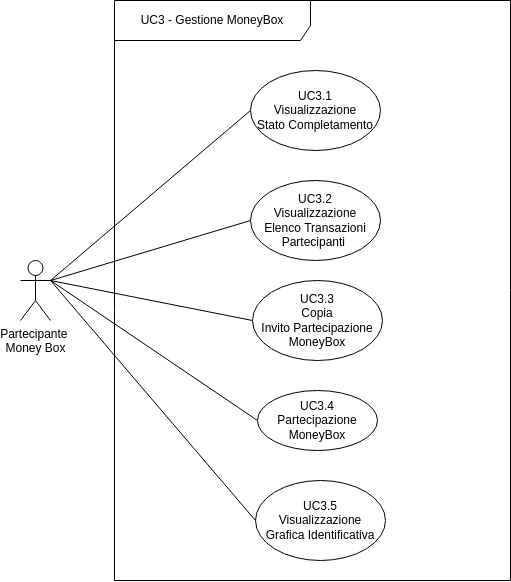
\includegraphics[scale=0.7]{immagini/UC3.png}
    \caption{UC3}
\end{figure}

\begin{itemize}
    \item Attore primario: partecipante MoneyBox;
    \item Precondizioni: il proprietario dell'ordine ha selezionato il pagamento MoneyBox\glo [UC2.2.2];
    \item Postcondizioni: il partecipante MoneyBox ha visualizzato i dati relativi la MoneyBox\glo{};
    \item Scenario principale:
          \begin{enumerate}
                \item Il partecipante MoneyBox può visualizzare lo stato del completamento in formato percentuale e il saldo mancante [UC3.1];
                \item Il partecipante MoneyBox può visualizzare un elenco delle transazioni partecipanti [UC3.2];
                \item Il partecipante MoneyBox può visualizzare l'invito per partecipare alla MoneyBox\glo{} [UC3.3];
                \item Il partecipante MoneyBox può partecipare alla MoneyBox\glo{} [UC3.4];
                \item Il partecipante MoneyBox può visualizzare una grafica identificativa della MoneyBox\glo{} [UC3.5].
    \end{enumerate}
\end{itemize}

\subsubsection{UC3.1 - Visualizzazione Stato Completamento}

\begin{itemize}
    \item Attore primario: partecipante MoneyBox;
    \item Precondizioni: il proprietario dell'ordine ha selezionato il pagamento MoneyBox\glo [UC2.2.2], 
            l'utente dispone dell'invito valido ad una MoneyBox\glo{} [UC3.3];
    \item Postcondizioni: il partecipante MoneyBox ha visualizzato lo stato del completamento;
    \item Scenario principale: il partecipante MoneyBox visualizza lo stato del completamento in formato percentuale e il saldo mancante.
\end{itemize}

\subsubsection{UC3.2 - Visualizzazione Elenco Transazioni Partecipanti}

\begin{itemize}
    \item Attore primario: partecipante MoneyBox;
    \item Precondizioni: il proprietario dell'ordine ha selezionato il pagamento MoneyBox\glo [UC2.2.2], 
            l'utente dispone dell'invito valido ad una MoneyBox\glo{} [UC3.3];
    \item Postcondizioni: il partecipante MoneyBox ha visualizzato l'elenco delle transazioni partecipanti;
    \item Scenario principale: il partecipante MoneyBox visualizza l'elenco delle transazioni partecipanti con i seguenti dettagli:
        \begin{itemize}
            \item Indirizzo del partecipante;
            \item Ammontare versato;
            \item Data di versamento.
        \end{itemize}
\end{itemize}

\subsubsection{UC3.3 - Visualizzazione Invito Partecipazione MoneyBox}

\begin{itemize}
    \item Attore primario: partecipante MoneyBox;
    \item Precondizioni: il proprietario dell'ordine ha selezionato il pagamento MoneyBox\glo [UC2.2.2];
    \item Postcondizioni: il partecipante MoneyBox ha visualizzato l'invito alla MoneyBox\glo{};
    \item Scenario principale: il partecipante MoneyBox visualizza l'invito alla MoneyBox\glo{}.
\end{itemize}

\subsubsection{UC3.4 - Partecipazione MoneyBox}

\begin{itemize}
    \item Attore primario: partecipante MoneyBox;
    \item Precondizioni: il proprietario dell'ordine ha selezionato il pagamento MoneyBox\glo [UC2.2.2], 
            l'utente dispone dell'invito valido ad una MoneyBox\glo{} [UC3.3];
    \item Postcondizioni: il partecipante MoneyBox ha selezionato la quota da versare e ha visualizzato la pagina di checkout;
    \item Scenario principale:
          \begin{enumerate}
              \item Il partecipante MoneyBox seleziona la quota da versare, compresa tra zero escluso e il minimo tra il saldo disponibile nel wallet\glo{} 
                    e il rimanente della MoneyBox\glo{};
              \item Il partecipante MoneyBox viene reindirizzato alla pagina di checkout con la quota scelta [UC2].
          \end{enumerate}
\end{itemize}

\subsubsection{UC3.5 - Visualizzazione Grafica Identificativa}

\begin{itemize}
    \item Attore primario: partecipante MoneyBox;
    \item Precondizioni: il proprietario dell'ordine ha selezionato il pagamento MoneyBox\glo [UC2.2.2], 
            l'utente dispone dell'invito valido ad una MoneyBox\glo{} [UC3.3];
    \item Postcondizioni: il partecipante MoneyBox ha visualizzato l'indirizzo della MoneyBox\glo{} come grafica identificativa;
    \item Scenario principale: il partecipante MoneyBox visualizza l'indirizzo della MoneyBox\glo{} come grafica identificativa.
\end{itemize}

\subsection{UC4 - Connessione Metamask}

\begin{figure}[H]
    \centering
    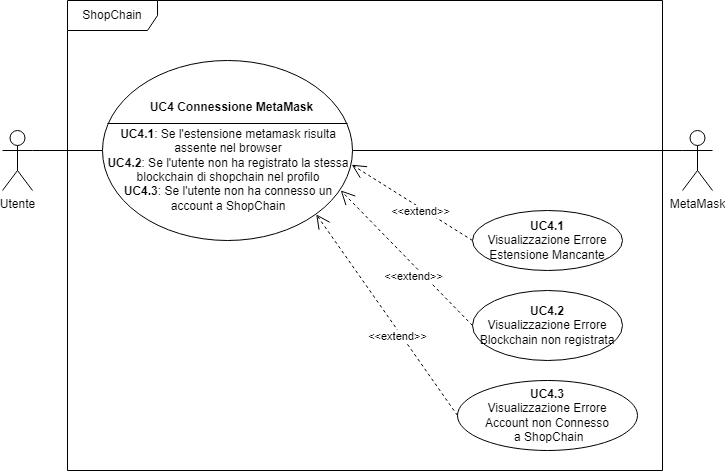
\includegraphics[scale=0.7]{immagini/UC4.png}
    \caption{UC4}
\end{figure}

\begin{itemize}
    \item Attore primario: utente generico;
    \item Precondizioni: il sistema è raggiungibile e funzionante;
    \item Postcondizioni: l'utente ha connesso Metamask\glo{} a ShopChain;
    \item Scenario principale:
        \begin{enumerate}
            \item L'utente visualizza il pop-up di Metamask\glo{} per la connessione a ShopChain;
            \item L'utente autorizza la connessione a ShopChain.
        \end{enumerate}
    \item Estensioni:
        \begin{enumerate}
            \item Nel caso in cui l'estensione Metamask\glo{} risultasse assente nel browser:
                \begin{itemize}
                    \item La connessione non ha successo;
                    \item Viene visualizzato errore estensione mancante [UC4.1].
                \end{itemize}
            \item Nel caso in cui l'utente abbia connesso il proprio wallet\glo{} ma non abbia configurato la stessa blockchain\glo{} di ShopChain:
                \begin{itemize}
                    \item La connessione non viene completata;
                    \item Viene visualizzato errore blockchain\glo{} non registrata [UC4.2].
                \end{itemize}
            \item Nel caso in cui l'utente non abbia connesso un account a ShopChain:
                \begin{itemize}
                    \item La connessione non viene completata;
                    \item Viene visualizzato errore account non connesso a ShopChain [UC4.3].
                \end{itemize}
        \end{enumerate}
\end{itemize}

\subsubsection{UC4.1 - Visualizzazione Errore Estensione Mancante}

\begin{itemize}
    \item Attore primario: utente generico;
    \item Precondizioni: l'utente utilizza un browser sprovvisto di estensione Metamask\glo{};
    \item Postcondizioni: l'utente ha visualizzato l'errore e la connessione fallisce;
    \item Scenario principale:
        \begin{enumerate}
            \item L'utente visualizza un messaggio di errore per mancata connessione;
            \item L'utente viene invitato a scaricare l'estensione Metamask\glo{};
            \item L'utente clicca ”OK” per continuare.
        \end{enumerate}
\end{itemize}

\subsubsection{UC4.2 - Visualizzazione Errore Blockchain non registrata}

\begin{itemize}
    \item Attore primario: utente generico;
    \item Precondizioni: l'utente ha connesso il proprio wallet\glo{} ma non ha configurato la stessa blockchain\glo{} di ShopChain;
    \item Postcondizioni: l'utente ha visualizzato l'errore e la connessione fallisce;
    \item Scenario principale:
          \begin{enumerate}
              \item L'utente visualizza un messaggio di errore per mancata connessione;
              \item L'utente visualizza i dati per configurare la blockchain\glo{};
              \item L'utente clicca ”OK” per continuare.
          \end{enumerate}
\end{itemize}

\subsubsection{UC4.3 - Visualizzazione Errore Account non Connesso a ShopChain}

\begin{itemize}
    \item Attore primario: utente generico;
    \item Precondizioni: l'utente ha configurato la stessa blockchain\glo{} di ShopChain ma non ha connesso un account;
    \item Postcondizioni: l'utente ha visualizzato l'errore e la connessione fallisce;
    \item Scenario principale:
          \begin{enumerate}
              \item L'utente visualizza un messaggio di errore per mancata connessione;
              \item L'utente viene invitato a connettere un account;
              \item L'utente clicca ”OK” per continuare.
          \end{enumerate}
\end{itemize}

\subsection{UC5 - Visualizzazione Indirizzo Wallet}

\begin{figure}[H]
    \centering
    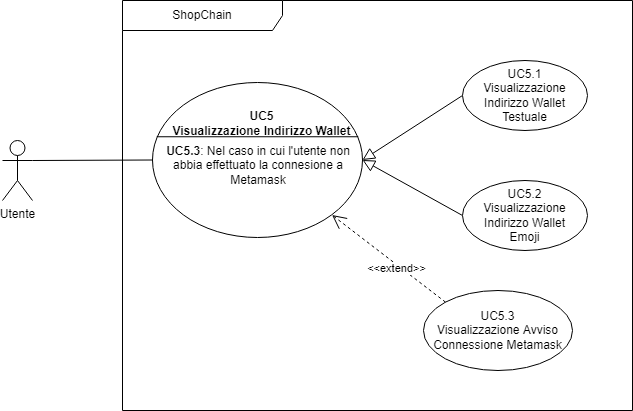
\includegraphics[scale=0.7]{immagini/UC5.png}
    \caption{UC5}
\end{figure}

\begin{itemize}
    \item Attore primario: utente generico;
    \item Precondizioni: il sistema è raggiungibile e funzionante;
    \item Postcondizioni: l'utente ha visualizzato l'indirizzo del wallet\glo{};
    \item Scenario principale: l'utente visualizza l'indirizzo del wallet\glo{}.
    \item Estensioni:
    \begin{enumerate}
        \item Visualizzazione Avviso Connessione Metamask\glo{} [UC5.3].
    \end{enumerate}
    \item Generalizzazioni: la visualizzazione dell'indirizzo può avvenire in maniera Testuale [UC5.1] oppure alternativamente sotto forma di Emoji [UC5.2].
\end{itemize}

\subsubsection{UC5.1 - Visualizzazione Indirizzo Wallet Testuale}

\begin{itemize}
    \item Attore primario: utente generico;
    \item Precondizioni: il sistema è raggiungibile e funzionante;
    \item Postcondizioni: l'utente ha visualizzato l'indirizzo del wallet\glo{} in forma testuale;
    \item Scenario principale: l'utente visualizza l'indirizzo del wallet\glo{} in forma testuale.
\end{itemize}

\subsubsection{UC5.2 - Visualizzazione Indirizzo Wallet Emoji}

\begin{itemize}
    \item Attore primario: utente generico;
    \item Precondizioni: il sistema è raggiungibile e funzionante;
    \item Postcondizioni: l'utente ha visualizzato l'indirizzo del wallet sotto forma di sequenza di emoji;
    \item Scenario principale: l'utente visualizza l'indirizzo del wallet sotto forma di sequenza di emoji.
\end{itemize}

\subsubsection{UC5.3 - Visualizzazione Avviso Connessione Metamask}

\begin{itemize}
    \item Attore primario: utente generico;
    \item Precondizioni: l'utente non ha effettuato la connessione a Metamask\glo{};
    \item Postcondizioni: l'utente ha visualizzato un avviso relativo la mancata connessione a Metamask\glo{};
    \item Scenario principale: l'utente visualizza un avviso relativo la mancata connessione a Metamask\glo{}.
\end{itemize}

\subsection{UC6 - Sblocco Ordine}

\begin{figure}[H]
    \centering
    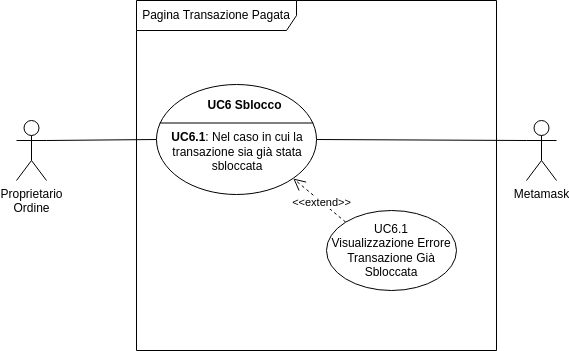
\includegraphics[scale=0.7]{immagini/UC6.png}
    \caption{UC6}
\end{figure}

\begin{itemize}
    \item Attore primario: utente proprietario dell'ordine;
    \item Attore secondario: utente venditore, Metamask\glo{};
    \item Precondizioni: il sistema ha generato il codice di sblocco [UC2.3.3];
    \item Postcondizioni: l'utente proprietario ha sbloccato l'ordine e il denaro è stato trasferito all'utente venditore;
    \item Scenario principale:
          \begin{enumerate}
              \item Il proprietario dell'ordine inserisce il codice di sblocco;
              \item Il proprietario dell'ordine conferma la transazione sul pop-up Metamask\glo{};
              \item Il sistema trasferisce il denaro sul wallet\glo{} dell'utente venditore.
          \end{enumerate}
    \item Estensione: Nel caso in cui la transazione sia già stata sbloccata:
          \begin{enumerate}
              \item Viene impedito lo sblocco;
              \item Viene mostrato un errore di Transazione Già Sbloccata [UC6.1].
          \end{enumerate}
\end{itemize}

\subsubsection{UC6.1 - Visualizza Errore Transazione Già Sbloccata}

\begin{itemize}
    \item Attore primario: utente proprietario dell'ordine;
    \item Precondizioni: il sistema è raggiungibile e funzionante, la transazione è già stata sbloccata;
    \item Postcondizioni: il proprietario dell'ordine ha visualizzato l'errore di transazione già sbloccata;
    \item Scenario principale: il proprietario dell'ordine visualizza l'errore di transazione già sbloccata.
\end{itemize}

\subsection{UC7 - Visualizzazione Transazioni}

\begin{figure}[H]
    \centering
    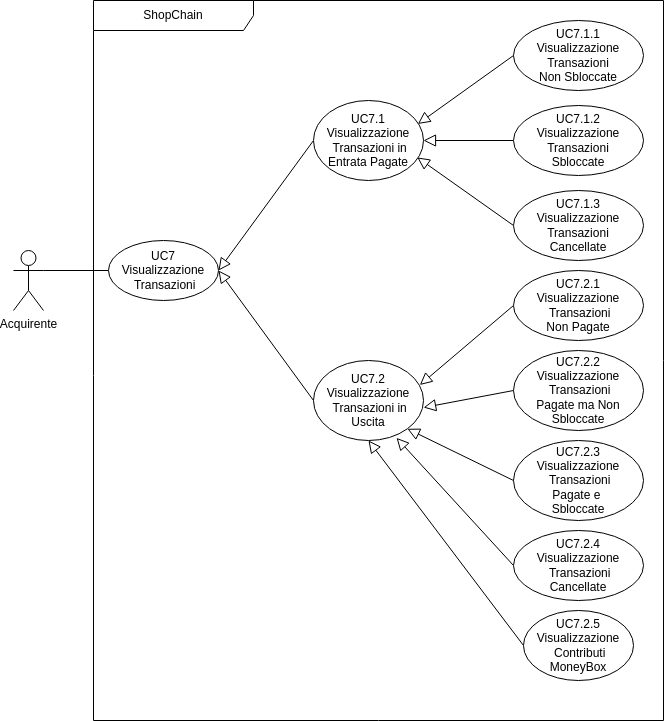
\includegraphics[scale=0.7]{immagini/UC7.png}
    \caption{UC7}
\end{figure}

\begin{itemize}
    \item Attore primario: utente generico;
    \item Precondizioni: il sistema è raggiungibile e funzionante;
    \item Postcondizioni: l'utente ha visualizzato le transazioni;
    \item Scenario principale: l'utente visualizza le transazioni con i seguenti dettagli:
        \begin{itemize}
            \item Codice Identificativo della transazione;
            \item Indirizzo venditore/acquirente;
            \item Ammontare pagato/da pagare;
            \item Stato dell'ordine;
            \item Data di creazione transazione.
        \end{itemize}
    \item Generalizzazioni:
          \begin{itemize}
              \item Visualizza transazioni in entrata pagate [UC7.1];
              \item Visualizza transazioni in uscita [UC7.2];
          \end{itemize}
\end{itemize}

\subsubsection{UC7.1 - Visualizza Transazioni In Entrata Pagate}

\begin{itemize}
    \item Attore primario: utente venditore;
    \item Precondizioni: il sistema è raggiungibile e funzionante;
    \item Postcondizioni: l'utente venditore ha visualizzato le transazioni in entrata pagate;
    \item Scenario principale: l'utente venditore visualizza le transazioni in entrata pagate con i seguenti dettagli:
        \begin{itemize}
            \item Codice Identificativo della transazione;
            \item Indirizzo acquirente;
            \item Ammontare pagato;
            \item Stato dell'ordine;
            \item Data di creazione transazione.
        \end{itemize}
    \item Generalizzazioni:
          \begin{itemize}
              \item Visualizza transazioni non sbloccate [UC7.1.1];
              \item Visualizza transazioni sbloccate [UC7.1.2];
              \item Visualizza transazioni cancellate [UC7.1.3].
          \end{itemize}
\end{itemize}

\paragraph{UC7.1.1 - Visualizza Transazioni Non Sbloccate}

\begin{itemize}
    \item Attore primario: utente venditore;
    \item Precondizioni: il sistema è raggiungibile e funzionante;
    \item Postcondizioni: l'utente venditore ha visualizzato la lista di transazioni non sbloccate;
    \item Scenario principale: l'utente venditore visualizza la lista di transazioni non sbloccate.
\end{itemize}

\paragraph{UC7.1.2 - Visualizza Transazioni Sbloccate}

\begin{itemize}
    \item Attore primario: utente venditore;
    \item Precondizioni: il sistema è raggiungibile e funzionante;
    \item Postcondizioni: l'utente venditore ha visualizzato la lista di transazioni sbloccate;
    \item Scenario principale: l'utente venditore visualizza la lista di transazioni sbloccate.
\end{itemize}

\paragraph{UC7.1.3 - Visualizza Transazioni Cancellate}

\begin{itemize}
    \item Attore primario: utente venditore;
    \item Precondizioni: il sistema è raggiungibile e funzionante;
    \item Postcondizioni: l'utente venditore ha visualizzato la lista di transazioni cancellate;
    \item Scenario principale: l'utente venditore visualizza la lista di transazioni cancellate.
\end{itemize}

\subsubsection{UC7.2 - Visualizza Transazioni In Uscita}

\begin{itemize}
    \item Attore primario: utente proprietario dell'ordine;
    \item Precondizioni: il sistema è raggiungibile e funzionante;
    \item Postcondizioni: l'utente ha visualizzato le transazioni in uscita;
    \item Scenario principale: l'utente visualizza le transazioni in uscita con i seguenti dettagli:
        \begin{itemize}
            \item Codice Identificativo della transazione;
            \item Indirizzo venditore;
            \item Ammontare pagato/da pagare;
            \item Stato dell'ordine;
            \item Data di creazione transazione.
        \end{itemize}
    \item Generalizzazioni:
          \begin{itemize}
              \item Visualizza transazioni non pagate [UC7.2.1];
              \item Visualizza transazioni pagate ma non sbloccate [UC7.2.2];
              \item Visualizza transazioni pagate e sbloccate [UC7.2.3].
          \end{itemize}
\end{itemize}

\paragraph{UC7.2.1 - Visualizza Transazioni Non Pagate}

\begin{itemize}
    \item Attore primario: utente proprietario dell'ordine;
    \item Precondizioni: il sistema è raggiungibile e funzionante;
    \item Postcondizioni: l'utente proprietario dell'ordine ha visualizzato la lista di transazioni non pagate;
    \item Scenario principale: l'utente proprietario dell'ordine visualizza la lista di transazioni non pagate.
\end{itemize}

\paragraph{UC7.2.2 - Visualizza Transazioni Pagate Ma Non Sbloccate}

\begin{itemize}
    \item Attore primario: utente proprietario dell'ordine;
    \item Precondizioni: il sistema è raggiungibile e funzionante;
    \item Postcondizioni: l'utente proprietario dell'ordine ha visualizzato la lista di transazioni pagate pagate ma non sbloccate;
    \item Scenario principale: l'utente proprietario dell'ordine visualizza la lista di transazioni pagate pagate ma non sbloccate.
\end{itemize}

\paragraph{UC7.2.3 - Visualizza Transazioni Pagate e Sbloccate}

\begin{itemize}
    \item Attore primario: utente proprietario dell'ordine;
    \item Precondizioni: il sistema è raggiungibile e funzionante;
    \item Postcondizioni: l'utente proprietario dell'ordine ha visualizzato la lista di transazioni pagate e sbloccate;
    \item Scenario principale: l'utente proprietario dell'ordine visualizza la lista di transazioni pagate e sbloccate.
\end{itemize}

\paragraph{UC7.2.4 - Visualizza Transazioni Cancellate}

\begin{itemize}
    \item Attore primario: utente proprietario dell'ordine;
    \item Precondizioni: il sistema è raggiungibile e funzionante;
    \item Postcondizioni: l'utente proprietario dell'ordine ha visualizzato la lista di transazioni cancellate;
    \item Scenario principale: l'utente proprietario dell'ordine visualizza la lista di transazioni cancellate.
\end{itemize}

\subsection{UC8 - Annullamento Ordine}

\begin{figure}[H]
    \centering
    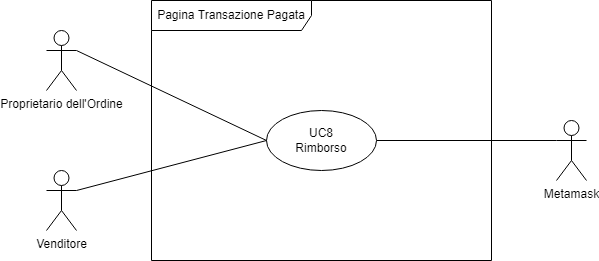
\includegraphics[scale=0.7]{immagini/UC8.png}
    \caption{UC8}
\end{figure}

\begin{itemize}
    \item Attore primario: utente venditore;
    \item Attore secondario: Metamask\glo{};
    \item Precondizioni: l'utente ha connesso il proprio Metamask\glo{} [UC4] ed esiste almeno un pagamento associato all'indirizzo dell'utente venditore;
    \item Postcondizioni: l'utente venditore ha annullato l'ordine e i fondi sono stati restituiti ai relativi acquirenti;
    \item Scenario principale:
          \begin{enumerate}
              \item L'utente venditore visualizza il pop-up di Metamask\glo{};
              \item L'utente venditore conferma l'operazione all'interno del pop-up;
              \item Viene annullato ogni versamento ed effettuati i rimborsi ai relativi acquirenti.
          \end{enumerate}
\end{itemize}

\subsection{UC9 - Richiesta Rimborso}

\begin{figure}[H]
    \centering
    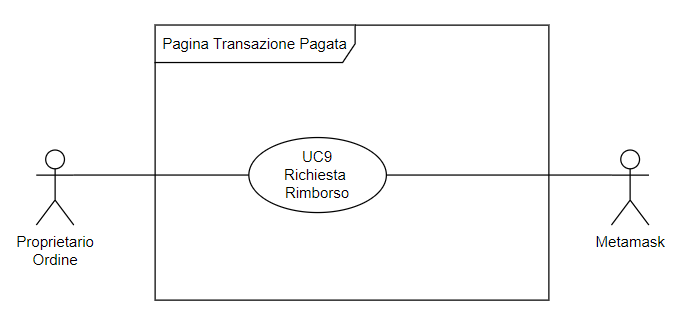
\includegraphics[scale=0.7]{immagini/UC9.png}
    \caption{UC9}
\end{figure}

\begin{itemize}
    \item Attore primario: utente proprietario dell'ordine;
    \item Attore secondario: Metamask\glo{};
    \item Precondizioni: l'utente ha connesso il proprio Metamask\glo{} [UC4] ed esiste almeno un pagamento associato all'indirizzo dell'utente proprietario dell'ordine;
    \item Postcondizioni: l'utente proprietario dell'ordine ha annullato l'ordine e i fondi sono stati restituiti ai relativi acquirenti;
    \item Scenario principale:
          \begin{enumerate}
              \item L'utente proprietario dell'ordine visualizza il pop-up di Metamask\glo{};
              \item L'utente proprietario dell'ordine conferma l'operazione all'interno del pop-up;
              \item Viene annullato ogni versamento ed effettuati i rimborsi ai relativi acquirenti.
          \end{enumerate}
\end{itemize}

\clearpage
